\newcommand{\idsystems}{\nedap Identification Services }
\newcommand{\nedap}{Nedap }
\newcommand{\ublox}{u-blox }
\newcommand{\sensit}{SENSIT }
\chapter{Proof of concept validation by case study}
\label{ch:validation}
This chapter will attempt to validate the applicability of the platform to the field of LPWA QoS monitoring and management. This will be performed by designing and developing a prototype monitoring application for a commercial car parking application sensor application. Firstly, some background will be given on the sensor application to be monitored. Next, the goals, claims and methodology of the study will be declared. With the goal and means stated, the experiment will be performed by realizing a prototype monitoring application. As the actual implementation details are auxiliary, they will not be examined in detail. However, the implementation will be described superficially to contextualize the validation efforts. After implementation, the results of the validation study will present and their implications deliberated. This chapter will be concluded with a discussion on the results, conclusions and limitations of the study.
\section{Context of the case study}
\subsection{Company background Background}
\label{sec:sensit}
\subsubsection*{Nedap - Identification Systems}
[TODO]
\subsubsection*{\sensit [smart parking] application}
The \sensit \idsystems smart parking application is devised to monitor parking lots and garages. It employ a huge amount (up to thousands) of affordable LPWA sensor nodes. Each individual parking spot is equipped with one of these sensors to determine its occupation. To determine changes in occupation, each sensor is equipped with an infra-red and magnetic induction sensor. Should a change in occupation be detected, a message containing the measured sensor deltas is sent to the back-end application. This granular approach to smart parking allows the \sensit application to monitor and visualise the occupation of individual parking spaces in a lot, garage or even across cities.

In order to communicate with the back-end the sensors employ wireless technology. Previously, the sensors were connected to sinks using a proprietary network of relay nodes. However the recent proliforation of large scale cellular IoT networks has caused \nedap to shift towards these technologies. This allows large numbers of sensors to a single cell tower, without the need of deploying and managing a network of relay nodes for new sensor deployments. Additionally the effort in managing and maintianing the network is outsource to professional operators. To connect the sensors to the internet the \emph{Narrow-band Internet of Things} technology was determined to be most suitable. New \sensit sensors are therefore equipped with \ublox \cite{web:ublox} NB-IoT radio modules to connect them to operated cell networks.

\subsection{Conceptualization of the monitoring application}
In this section we will describe and scope the context of the QoS monitoring application to be developed. We will first describe the input for the application in terms of sensor data emitted by the WSN application under investigation. Consequently, the characteristics of the expected outcomes of the application to be prototyped will be discussed. 

\subsubsection{Sensor data signature}
The sensor devices send a message with key point information (KPI) data along with every data message it sends. Alternatively, it will send one of these messages periodically if no data messages are sent for [time period]. When computed universally, a message rate was determined of about 15 messages per sensor per day. However a specific per sensor analysis yields a message rate of between 10 and 50 KPI information messages on average per day, with some outliers for more active sensors which can reach up to 250 messages per day on a regular basis.

The data sent by the sensor contains some typical networking data points, such as source IP address, source port, source device ID, message sequence number and a timestamp. Additionally the message contains a hexadecimally encoded string describing the KPI's collected by the \ublox radio module. The data collected by the \ublox module contains mostly data points depicting the signalling functions of the radio module. Such KPI's include the signal-to-noise ratio, signal quality (RSSI), Extended Coverage Level (ECL)  and more. Additionally the KPI information includes some physical attributes of the radio module. Attributes such as the module's uptime, number of restarts and temperature. 

%TODO recalc nr byts!!!!
The ordinary data plus the \ublox KPI data are contained within [128] bytes of data (\nicefrac{1}{2} KiB). Considering the messaging rate of a typical sensor we yield an imposed per sensor footprint on bandwidth of 5-25 KiB/day for the majority of sensors, with outliers of 125 KiB/day for extremely active sensors.

At this moment only a few nodes equipped with the NB-IoT technology have been deployed. Therefore a large scale test bed for the to be prototyped monitoring application does not exist. Therefore a simulated sensor environment has been devised to test the prototype application for contemporary and near-future smart parking applications. This simulation is based on data signatures and values observed over a half year period emitted by the few nodes that have been deployed.

\subsubsection{QoS monitoring needs}
In collaboration with \idsystems a list of requirements for the outcomes of the prototype was compiled. These consequences are to be effected by the prototype application, based on input from (simulated) sensors. However, the actual implementation of the prototype is secondary to this chapter, since the primary goal is to evaluate choices made for the underlying development platform. Therefore a comprehensive, formalized requirements document has not been included in this thesis. We will however shortly describe the features required of the monitoring application to be developed in order to contextualize the implementation efforts of the prototype.

The consequences the application must effect are classified into three categories. The first of which is sensor feedback. This entails commands sent to sensors to alter its execution strategy, based on observations made in the monitoring application. This can be based on individual sensor data, historic sensor data or higher level data snapshots (e.g. sink level). An example of such feedbacks are to decrease data rates to guarantee a predetermined minimum sensor lifetime or due to poor cell connectivity. This functionality is currently not present in the \nedap sensors, but is intended in the future. Therefore it will be implemented into the simulation environment to test the command \& control capabilities of the platform.

The second type of effect to be caused by the application is instant alerting. The primary use case for this kind of consequence is when physical maintenance is imminently required in the application or its network. Detectable causes of when this might be warranted have been deliberated with \idsystems and examples include:
\begin{itemize}
\nospace
\item a long term drop in coverage level which might indicate permanent obstruction of signal
\item extremely high temperature readings indicating an electrical malfunction
\item unusually long periods of inactivity or, conversely, extreme data bursts indicate a rouge node not executing according to a valid strategy.
\item calculations estimating node lifetime determining a node needs replacing.
\end{itemize}

The last type of consequence is reporting. The goal of this is to inform technicians, managers or clients on the general operation of the WSN application. This comprises two types of reporting. The first is \emph{periodical reporting}. Periodical reporting will primarily focus on business goals such as long term performance metrics, compliance to service level agreements of both service providers and clients, and prospected short-term maintenance efforts and costs. The other type of reporting is \emph{real-time reporting}. This is useful to technicians monitoring the performance of an application during its runtime. Use cases include monitoring the number of incoming events, latencies of sensor devices and sinks, environmental conditions (such as weather and temperature) and which sensor strategies currently are deployed. Notice that the real-time aspect of this type of reporting does not require events to be reported instantaneously since for such statistics a per second or minute update suffices.

%\section{Structure of the validation study}
%With the application, case and its context clear, the focus will be turned to detailing the validation study. Before executing our validation study, this section will first depict the taken process. We will begin by clearly stating the claims we aim to confirm and the bounds of our scope. Following that we will describe the intended method of testing those claims specifically by detailing the quantified criteria the platform implementation process must adhere to. We must note that these criteria will only cover the scope of the validation study, not the functional requirements of the implementation for the case. As mentioned before, though important for the outcome of the product for the company, for this validation study these requirements are ancillary.

%With the goals clearly stated, parametrized and quantified, we will design and implement a prototype monitoring application built upon the developed software platform, tailored to the QoS monitoring needs of \idsystems. As mentioned before the actual implementation details are secondary for validation purposes of this chapter. Therefore we will only touch upon it shortly without going into great detail. We will however give a short summary of the developed prototype to provide a context to the validation efforts. During and after the development process we will measure the relevant parameters required to evaluate the determined validation criteria. To conclude the investigative implementation, we will attempt to adapt the constructed application to a few hypothetical extension scenarios in order to explore the adaptability of the provided platform.

%We will conclude this chapter by stating, analysing and deliberating the results obtained by measuring and observing the development process. These results will be compared with the priorly determined criteria of the study. If these criteria are met, this will validate the claims they are meant to affirm. We will finish by discussing the process and results in order to deliberate the limitations and lessons learned regarding the proposed development platform.
	
%\section{Criteria of the Case Study}
\section{Method}
\label{sec:val:method}
\subsection{General approach} 
In order to validate weather the level of abstraction of the platform can facilitate the needs of the intended monitoring application for \sensit, a prototype implementation will be designed and constructed. The expected outcome is an instantiation of the platform that serves the QoS processing needs The possible existence of such an instantiation demonstrates that, at least for this use case, the level of abstraction is low enough to expose the full functionality that is required  (\textbf{applicability}). In order to validate that the level of abstraction is low enough, but not too low (\textbf{usability}), we will consider the program instructions required for the platform instantiation. These required instructions should not be more then the instruction required for a hypothetical monolithic implementation, supposing the level of abstraction is not too high (applicability claim). Finally, the \textbf{adaptability} of the platform and its instantiations will be evaluated by introducing some minor new features and requirements to the platform implementation. Should the appropriate level of abstraction have been chosen, it should prove uncumbersome to adapt the topology to these novel conditions.

From a business perspective, the most interesting parameter to express the adoption effort would be the time required to develop and evolve an application based on the proposed technology. However, this parameter is extremely subjective as it heavily depends on the level of skill of the developer and its familiarity with the technology. We will therefore primarily measure the effort by the code, expressed in number of instructions, required to construct a monitoring application built by integration of our platform. 
%TODO voor presentatie: goldylocks area.

\subsection{Claims}
\label{sec:claims}
In this section we will state the claim and criteria regarding the proposed platform we aim to validate. The cardinal claim investigated is that the appropriate level of abstraction was chosen in the design of the development platform. This entails that our collection of components can be adapted to suit a plethora of purposes and target applications. Conversely, the level of abstraction is not that low-level that every implementation requires unnecessarily large development efforts because basic procedures require repeated implementation. This claim mirrors the research question \ref{rq:abstraction}, which asks "What is the appropriate level of abstraction for a WSN monitoring platform [...]". This claim is explicated into three sub-claims.

\subsubsection{Applicability}
Intuitively, the first criterium regarding the level of abstraction is that the platform features a level of abstraction low enough to facilitate the implementation of the monitoring application for \sensit. I.e. the platforms abstraction does not obfuscate key functionalities which would require reimplementation of formerly present features. This seems an obvious and trivial demand, but without stating it, any subsequent criterium is pointless. More specifically, the platform should enable an instantiation which enables iterative and consequent enrichment and accumulation of information. At multiple stages of the consequential iteration the application should be able to generate outputs such as alerts and reports for auxiliary processes and systems.

\subsubsection{Usability}
The second criterium to be validated is that the level of abstraction is not too low. Though the platform should enable an instantiation according to the needs of \idsystems, it should do so with minimal development effort. A [too low] level of abstraction requires application developers to repeatedly implement functionality that, due to their frequent nature, should have been provided by the platform itself. This criterium seems similar to the first, but the metrics determining their attainment are measured differently. Therefore, they will be regarded as two separate claims.

These development efforts will be expressed in the number of code instructions required to realize the implementation. Since an absolute benchmark was difficult to ascertain, the upper bound of permissible number of code instructions is established relative to the amount of instructions necessary for a functionally similar monolithic implementation. Should a larger code-base be determined, this entails a level of abstraction that is too low and requires (repeated) implementation of procedures that should have been provided by the platform itself. For the construction of the topology it was chosen to allow at most 4 operations for every component in the platform topology. The parameter of 4 operations per component originates from an assertion made in Chapter \ref{ch:architecture}.

\subsubsection{Adapatability}
The final criterium employed to validate the appropriate level of abstraction is that the platform facilitates convenient adaptation of a realized platform implementation. This validation will be performed by introducing or changing a minor feature (e.g. new input type, altered reporting requirement). Should the appropriate level of abstraction have been chosen, it should prove uncumbersome to adapt the topology to these novel conditions. For the adaptability of the application provided by the platform it was determined that minor new features and requirements should require not more than
\begin{itemize}
\nospace
\item a localized rearrangement of the model/topology, 
\item introduction or major change of at most two components, 
\end{itemize}
As for all cases, small changes are allowed to the components interfacing with the altered component(s) in order to produce or consume information supplied to or emitted by the altered component. Additionally, we allow for very minor, consistent changes to be made to other components. The reason for this is that often a change or introduction of a datapoint requires that change to be forwarded throughout the topology.

The rationale for these allowances is that the modularization provided by the platform should prevent entanglement of concerns and therefore minor changes should cause localized effects. There is however a possibility that (especially new features) require a change in several components since its the functionality was not previously present. Therefore minor consistent changes are allowed to those components in order to forwarded the new functionality. Finally, the reason for the allowance of a major change in two components is that often computation and analysis of a datapoint is separated into distinct components due to separation of concerns. Therefore a changed requirement will often require a change in both components.

%To recap, we validate the main claim by three sub-claims that are summarized as applicability, usability and adaptability. For the remainder of this chapter these three claims will be addressed using these headings. In full these claims read:
%\begin{description}[style=nextline]
%\nospace
%\item[Applicability] The platform's level of abstraction is low enough to suit a large number of applications,
%\item[Usability] The platform's level of abstraction is high enough that the framework prevents repeated implementation of common procedures, and
%\item[Adaptability] The platform facilitates effortless adaptation of an instantiated application.
%\end{description}
%Altogether, these claims culminate in the main claim that the appropriate level of abstraction has been chosen.

\subsection{Bounds}
Before executing the validation study, the bounds and limitations of this validation study will need to be considered. The first glaring limitation of this study is that it is extremely limited in scope. The platform will only be implemented for a specific WSN application and this study will therefore not state the platform to be appropriate for the entire set of applications that was determined in Section \ref{sec:back:context} of the background chapter. Instead, this study will at most affirm the platform as a proof-of-concept for WSN application QoS monitoring.

The second limitation worthy of notion is that, aside from only regarding a single WSN application, it will also run on a simulation of that application. As mentioned before, this is because the NB-IoT incorporated sensor devices of the \sensit application have only recently started deployment. As a consequence a test bed of significant scale is presently not available. However by simulating a full future deployment of the application we are able to easily adapt the WSN application under investigation, in terms of both scale and functionality. This allows us to not only test for intended regular behaviour but also for extreme and niche conditions. Additionally our simulated environment allows for easy temporal manipulation, which enables us to speed up, halt and repeat simulations.

%only one case. Partial validation, proof of concept
%simulated environmant (based on acutal data signatures and data rates)
%	current state of sensit not a scale challenge
%	simulation can fast forward

%\subsubsection{Summary of criteria}
%The concrete criteria formulated in this section are as follows:
%\begin{enumerate}
%\nospace
%\item An instantiation of the proposed platform should be possible in accordance with the needs and wants of \idsystems, which allows for
%\begin{itemize}
%\item iterative and consequent enrichment and accumulation of information, and
%\item output consequences at multiple stages of computation.
%\end{itemize}
%\item The instantiation of the platform should require 
%\begin{itemize}
%\item no more calculation code than it would in a monolithic system, and
%\item at most 4 instructions of code per component to build the topology.
%\end{itemize}
%\item A minor change in the goals or requirements should require only one change in the topology, a single component (and its interfacing) or a small and consistent change in multiple components.
%\item A realistic deployment of the instantiated application should be able to handle an input of 100.000 devices.
%\item A reconfiguration of the realistic deployment should be able to handle a hypothetical load of 1 million input devices, without changing the topological order of the components.
%\item An event burst of factor 100 should be processed within [number] seconds.
%\end{enumerate}

%Aside from the usability criterium we find the scalability required of the platform. We will formalize this requirement with two criteria. The first regards the general scalability of the platform. It requires the application to be able to cope with fantastic amounts of input data by only reconfiguring the worker tasks of the application, without changing the topological order of those components. Secondly, the implementation should be able to cope with fluctuating data signatures. For this the following criterium was formulated. The platform implementation should return to normal execution parameters within a certain amount of time after experiencing an increased input load.

%\subsubsection{Criterium parameters}
%While the functional criteria pose a binary decision on pass or fail, the non-functional criteria require quantification in order to determine weather they hold for the platform implementation. These parameters are based upon contemporary and near-future use cases and have been determined in collaboration with industry experts of \nedap. For the usability requirement it was chosen to express them in the number of instruction required. As an absolute upper bound on the amount of code proved to be difficult to determine before-hand, it was defined as "the amount of instructions and computations required for calculating the QoS parameters in a monolithic application, plus at most 4 lines of code for every component in the platform topology". The parameter of 4 lines of code per component originates in assertion made in Chapter \ref{ch:architecture}.

%For the adaptability of the application provided by the platform it was determined that minor new features and requirements should require not more than
%\begin{itemize}
%\nospace
%\item a localized rearrangement of the model/topology,
%\item introduction or major change of at most two components, 
%\end{itemize}
%As for all cases, we allow small changes to the components interfacing with the altered component(s) in order to produce or consume information supplied to or emitted by the altered component. Additionally, we allow for very minor changes to be made to other components. The reason for this is that often a change or introduction of a datapoint requires that change to be forwarded throughout the topology.

%The rationale for these allowances is that the modularization provided by the platform should prevent entanglement of concerns and therefore minor changes should cause localized effects. There is however a possibility that (especially new features) require a change in several components since its the functionality was not previously present or necessary. Finally, the reason for the allowance of a major change in two components is that often computation and analysis of a data is separated into distinct components due to separation of concerns. Therefore a change requirement will often require a change in both components.

%Finally, for the scale of the input signature for the monitoring application, the realistic near-future scale of the sensor application was determined to be 100.000 devices. For the fantastical size of future applications we have taken an increased factor of $\times$10, i.e. 1 million devices. Finally, for the increased signature of the temporary event shower to be processed we have chosen a factor of $\times$100 of the realistic data signature. This burst is supposed to be processed within one minute, after which the application should return to regular execution parameters.




%functional
%	features
%	not measurable, just attainable
%	- multilevel reporting
%	- enrichment through platform
%non-functional
%	scale 
%		x sensors
%	ease-of-implementation
%		1 fte week
%	measurable
%	validation criteria
	
\section{Implementation of the WSN monitoring application}
\subsection{Design and Implementation}
In this section the design for the \nedap \sensit and its implementation details will be described. We will first take a top-down look at the entire topology. After which we will shortly describe the functionality of the individual components.

\subsubsection{Application topology}
The designed topology is depicted in Figure \ref{fig:sensit_topology}. From this we see that the processing is divided into three stages. In the first stage raw-information snapshots are enriched and normalized. In doing so it improves the information potential and accuracy of the data in the snapshot. The second stage concerns sensor level analysis and management. It calculates the state and resource consumption of the devices, and it includes some services that alert if a sensor exhibits abnormal behaviour or long term deviations of its ordinary parameter margins. The final stage concerns snapshot accumulation in order to extract high level information and decisions from it. This stage diverges into three distinct accumulator paths. The top path performs accumulations of snapshots based on the sensor group ID. It reports on data rate violations (as agreed upon in SLA's) and recalculates the share of the data each sensor within a sensor group is allowed to consume. The middle execution path concerns the cells served by nodes. It alerts if a node switches cells more then an allowed amount during a period. The bottom accumulates all the snapshots in order to report on the current state of the application as a whole.

\begin{sidewaysfigure}
\centering
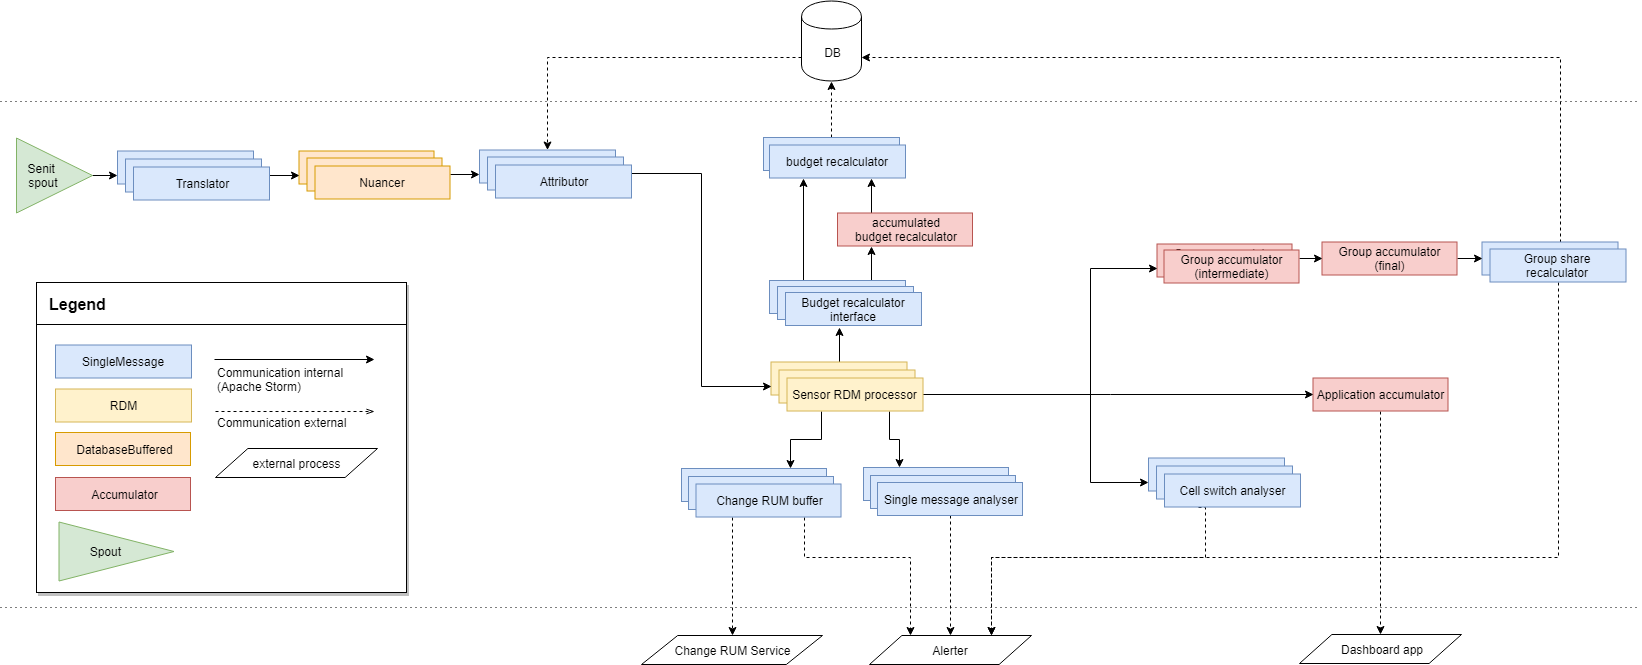
\includegraphics[width=1.15\textwidth]{resources/img/sensit_topology.png}
\caption{Topology of the monitoring application for the \idsystems \sensit WSN application}
\label{fig:sensit_topology}
\end{sidewaysfigure}

We will conclude the description of the application topology by shortly describing the functions of the individual components.
\begin{description}[style=nextline]
\nospace
\item[Sensit spout] Reads sensor snapshots from a Kafka channel and introduces them into the topology.
\item[Translator] Translates the sensor information from hexadecimal string to key-value pairs.
\item[Nuancer] Averages the data points received from a sensor to eliminate abnormalities. It does so by keeping a record of the last seen messages for each sensor node in an SQL database.
\item[Attributor] Enriches the snapshot with some datapoints not present in the sensor but known by  back-end applications.
\item[Sensor RDM processor] Processes the enriched information from the snapshot and calculates the optimal operational device strategy.
\item[Switch strategy buffer] Buffers the switch strategy messages to prevent superfluous, erratic feedback to the sensors. Doesn't switch strategy on first report, only if a switch is requested over an extended period.
\item[Single message analyser] Calculates weather the sensor parameters (as calculated by the RDM processor) are within the allowable margins.
\item[Budget recalculator interface]If the message rate of a sensor is high enough will initiate an immediate budget recalculation. If message rate is low it is allowed to be accumulated over some time to reduce the number of database updates.
\item[Budget recalculator accumulator] Accumulates budget recalculation snapshots and prepares them  for batch update.
\item[Budget recalculator] Executes batch budget recalculation.
\item[Group accumulator] Accumulates snapshots by sensor's group ID. Because this is performed on a weekly basis, this is performed two-stage as not to cause a large data build-up over time.
\item[Group share recalculator] Recalculates the share of the sensor group's resources each sensor is allowed to consume, based on the data used by each node over a one week period.
\item[Application accumulator] Accumulates the information emitted by the application in order to be presented on an application dashboard.
\item[Cell Switch Analyser] Analyses and reports if a node switches between cell towers more then is allowed.
\end{description}

Final remark on the application design is on the interfaces it provides. The application's inputs and outputs received and provided to Apache Kafka channels. This allows actual services to be easily swapped in and out with test services (even at runtime). 

\subsubsection{Sensor Resource Distribution Model}
To model the state, behaviour and strategies of the sensor we employed the RDM model proposed in Chapter \ref{ch:rdm}. The resulting model is depicted in Figure \ref{fig:sensit_rdm}. The model takes a few parameters based on the sensor state measurements, such as its current ECL and message rate, and its history, such as its runtime, data already used and budget already used. The model then computes the runtime the sensor has left, current data and budget consumption and the optimal mode of operation. By optimal we mean the operational strategy with the highest message rate that will not exceed the resource availability.

\begin{figure}
\centering
\hrule
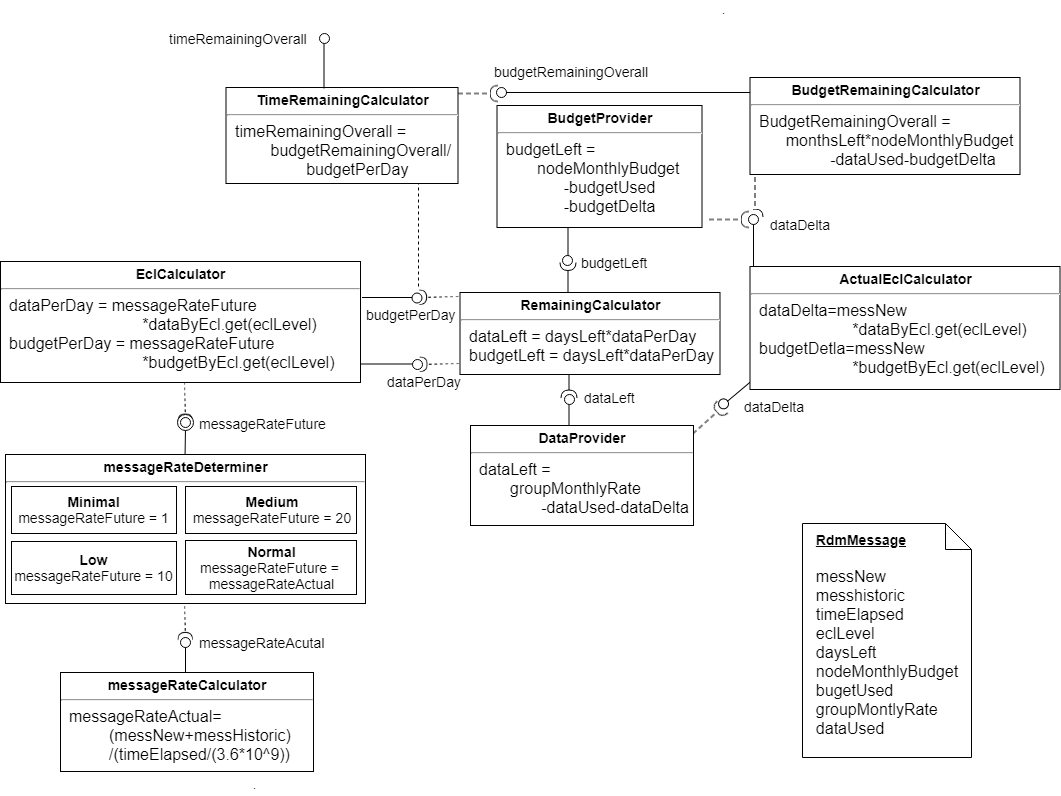
\includegraphics[width=\textwidth]{resources/img/sensit_rdm.png}
\hrule
\caption{Resource Distribution Model for a sensor in the \idsystems \sensit WSN application}
\label{fig:sensit_rdm}
\end{figure}

Earlier experiments with resource consumption models have shown that a device will act differently when in the beginning than in the end of its life-cycle, when there is a scarce resource involved. The reason for this is that in the beginning the models will instruct the device to operate on a strategy that will consume less resources then it is allowed on average. Then, when it has saved up enough of that resource, it is allowed to spend it on a strategy that consumes more than that average. To mitigate this effect is has been chosen to recalculate the available resources on a monthly basis. This way there is still such a cycle, but its period is far shorter and the effect will be much less and much more regular overall.

\subsection{Adapting the application}
We will conclude this section by deliberating some hypothetical adaptations in order to investigate the adaptability of the platform.

\subsubsection{Nuancer local}
The first change we introduce is the constraint for the \emph{Nuancer} to not require a database connection. Reason for such a requirement is to reduce latency or to eliminate capacity issues caused by employing an SQL database. 

This can be achieved by exchanging the current \emph{DatabaseBuffered} Nuancer implementation with a \emph{SingleMessageProcessor}. This processor keeps an in-memory cache of the last snapshots it has encountered, grouped by node and ordered by timestamp or sequence number. For each incoming snapshot the following sequence of actions is taken:
\begin{enumerate}
\nospace
\item determine node by ID,
\item add snapshot to the node's buffer,
\item purge out-of-scope snapshots from the cache,
\item calculate average of remaining buffered snapshots, and
\item emit averaged snapshot
\end{enumerate}
This sequence of actions is similar to how the Nuancer operates in the current topology, but it eliminates the database connection in favour of a local buffer of snapshots. Unfortunately by shifting to a local buffer we can no longer employ the scaffolding provided by the \emph{DatabaseBufferComponent}. The reason for this is that the component with local buffer (as currently implemented) operates on a single global buffer, instead of a buffer per node.

Finally, it must be noted that in requiring the snapshots to be cached locally, a large burden is forced upon the memory of the machine running the component. Should the application serve a large amount of nodes and snapshots are collected within a large window if interest, the data kept in-memory can rapidly reach large sizes. This can be alleviated by replicating this component to the point that individual memory requirements of workers are within manageable parameters. Alternatively, the memory issue can be evaded by persisting and reading snapshots to local files. This introduces some latency due to disk IO, but can immensely reduce the number of records in the active cache at any time.

\subsubsection{New sensor data encoding}
As mentioned, the auxiliary performance data of the sensor is received as an encoded hexadecimal string. For this case we introduce a new type of sensor equipped with a different radio module, which encodes its performance datapoints slightly differently. Though deliberated as a hypothetical, this case simulates a real future scenario. Since the aim is for a node lifetime of at least 10 years, it is very conceivable that sensor wireless technologies improve and change during that timeframe. Since physical replacement of the large volumes of deployed nodes is unprofitable for both \nedap and its clients, this new technology should be supported in tandem with the old sensor types. We emphasize that for this case we do not significantly change the actual data collected and emitted by the device as this would entail a major change in how computations need to be performed.

This change in the sensor environment can be accommodated for by introducing a second \emph{Translator} component specifically intended for the new data format. This component is executed independently of, and in parallel to, the original Translator. How to ensure that a snapshot is processed by the correct translator, will depend on how the new the data stream is supplied to the application. For this hypothetical we will consider the most complicated input option, where the old and the new style snapshots are emitted on a single input channel. To split the singular input stream into two an interface component is introduced. This component performs a superficial inspection of the snapshot and forwards it to the correct Storm channel based on some discerning feature (format, type identifier, etc.). Though technically this inspection could be performed by the \emph{SensorSpout}, separation of concerns compels a separate component for this purpose. Subsequently, both translators uniformly emit their translated snapshots to a common Storm channel for further processing. The resulting partial topology is illustrated in Figure \ref{fig:update_encoding}

\begin{figure}
\centering
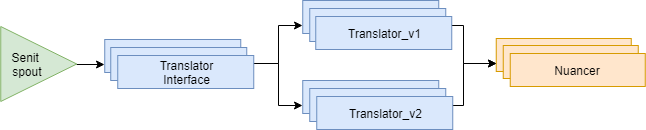
\includegraphics[width=0.7\textwidth]{resources/img/update_encoding.png}
\caption{Updated partial topology for new data encoding}
\label{fig:update_encoding}
\end{figure}

\subsubsection{Alert on long-term ECL drop}
For our final case we extend the functionality of the application by introducing a new outcome for the application. The added requirement is the detection of long term drop in ECL level. Such a drop could signify a, possibly alleviable, obstruction placed between the sensor and the sensor sink. Moreover, should several geographically related sensors report such a disruption, drastic actions cannot be ignored. In our topology this can easily be achieved by extending one of the existing components. Formally, the \emph{CellSwitchAnalyser} would be most suited for this purpose, since it is already historically aware due to retaining a list of cell towers per sensor. Though the component would obviously require renaming.

We provide this functionality by keeping a list of ECLs reported by each sensor node. When the sightings are inconsistent or do not feature a drop, the list is purged. When the list's size (or timestamp difference) surpasses a set threshold, an alert is sent to the alerter. This is easily performed since the CellSwitchAnalyser already features alerting functionality. Finally this change does not require changes to interfacing components, since the ECL level is already present in the snapshot emitted by the \emph{SensorRdmProcessor}.

\section{Results}
We will report the results under their own three headings: applicability, development effort and adaptability

\subsubsection{Applicability}
The sensor model was found to be adequate for modelling the behaviour of the \sensit sensors. The modular design proved very useful for expositioning the different resources and how they were interconnectively calculated and distributed. Unfortunately (for the purpose of this study), the sensor did not feature a large variety of resource metrics specifying its configurable behaviour and therefore the model only featured one configurable component. Additionally, after accumulation of the application-level parameters by the \emph{ApplicationAccumulator} the accumulated parameters needed no further transformations and the WSN application did not feature application-level configuration needs. Therefore the Resource Distribution Model was only employed on the sensor-level.

The result of the applicability investigation with regard to the distributed topology is that the platform suffices as development platform for the purposes of \idsystems. The building blocks provided enable the implementation of a functional application and provides functional abstraction of the specifics of the underlying technologies.  During implementation of the application it was noted however that the platform does not provide an efficient way of buffering and processing snapshots grouped per node, cell tower, etc. 

\subsubsection{Usability}
%It took about 80 hours to conceive, implement, debug and tune this architecture implementation. This time spent can be divided into roughly 15\% design, 35\% initial implementation and 50\% debugging and tuning \footnote{All hours spent on a component after its first inclusion in the topology and executing it are pooled into the latter category}.
%TODO model requirements res+comp+interf+rdm*connRes
Specifying the sensor model and application topology could be performed within the set parameters. As claimed, each component requires but four actions to be introduced to the topology. These actions are create component, declare component, subscribe consumer channels, declare output channels.

However the internal code of the topology components, which actually performs the calculations and computations, required about twice the amount of code that a monolithic application would. While the actual number of lines of code was only a little higher than then its monolithic counterpart would, the computations and transformations performed on those lines was far more then would be necessary in a monolithic application. These discrepancies will be deliberated on further in Section \ref{sec:eval}.

\subsubsection{Adaptability}
Finally, the necessary adaptations to the existing application for each hypothetical case are summarized in Table \ref{table:adaptations}.

\begin{table}
\centering
\begin{tabular}{|l||c|c||c|c|} \hline
Summary				& \multicolumn{2}{c||}{Components}		& \multicolumn{2}{c|}{Topology changes} \\ 
					& new 	& changed 	& none 		& only local  \\ \hline 
Nuancer local		& 0		& 1			&			& \cmark \\ \hline
New sensor encoding	& 2		& 0			& 			& \cmark \\ \hline
Alert ECL drop		& 0		& 1			& \cmark	&		 \\ \hline
\end{tabular}
\caption{changes required per adaptation scenario}
\label{table:adaptations}
\end{table}

%Applicability
%	goed, mist mapped-buffer
%2x zolang als gepland
%	tracability difficult
%	disjunction 2d model, 1d coding
%	debug first run duurt lang want string-bindings en string serialized
%	part testing is goed (dump result/intermediate)
%	solved by structs
%Meer code dan gepland (bijna 2x zovel)
%	building models en topology wel goed
%	(de)serializing
%	solved by structs
%[todo:timing/scalability]
\section{Evaluation}
\label{sec:eval}
In this section we will evaluate the obtained results and compare them to the criteria set out in section \ref{sec:criteria}. The criteria will be deliberated in the same order as the results in the previous section were.

\subsubsection{Applicability}
As stated, the building blocks provided by the platform allowed for a sufficient implementation of the intended monitoring application. However it was discovered that, though possibly useful, the platform did not provide an efficient template to buffer snapshots grouped by a certain snapshot parameter.  This component could easily be provided by introducing a mapper function to the \emph{BufferedProcessor} which will determine into which buffer a snapshot will be added to. The existing filter, sort and execution methods will then be performed on these buckets individually, providing a mechanism of grouped computations.

However such functionality currently is not present, this absences was easily avoided and was found to be only a minor inconvenience. Since this issue singularly was not sufficient to invalidate the applicability criterium we state that Criteria 1-3 hold.


\subsubsection{Usability}
%As mentioned it took about 80 hours to construct an develop the prototype application. This is twice as many as was originally stated in the validation criterium (Criterium 4). 
As mentioned in the results, though the code required to compose the resource models and application topology was contained within the specified parameters, the code required for the internals was found to be significantly more than a monolithic application would require. We therefore yield that \emph{usability} criterium was invalidated. The chief reason that the component internals required  more instructions as required in a monolith is the repeated serialization an deserialization of data into messages. Processing of each (group of) snapshot(s) is prepended with a few lines of code that extract, parse and cast each individual variable from the snapshot. After the component's processing is performed, a new snapshot is prepared with variables that again require its values to be serialized. When the computations of a component only amount to a few lines of code, this (de)serialization can quickly require more code than the actual computations do.

This was also reflected in the time required to develop this prototype. It was initially expected that the instantiation could be constructed within 40 man hours. However, this eventually took twice as many hours. Of that time about 15\% was spent designing, 35\% developing and 50\% debugging the application\footnote{All hours spent after fully constructing and first execution of the application are pooled into the latter category}. When we inspect the breakdown of the time spent we yield that it took an enormous amount of time to debug and adapt the components after its original design and implementation. The chief reason for this was found to be the loose coupling between components. The components are completely disjoint and the snapshot variables they share require custom serialization in between components and accessed with string identifiers. This entails that it is excessively easy to implement a broken component. This is since inappropriate variable access due to misspelled identifiers can occur very easily and is not detected by code checkers and compilers of conventional IDEs. Subsequently, when the variable is accessed successfully, the value often requires deserializing into the correct primitive or object type. This again introduces a possible point of failure due to misparsing and miscasting, since the compiler cannot detect the actual object type without executing the application.

To alleviate both the above mentioned problems we propose the introduction of snapshot struct objects (POJOs). These objects contain the variables of the snapshots passed between components. However, in contrast to loosely coupled key-value bindings, these bindings are explicitly defined in both type and identifier. They can therefore easily be serialized and deserialized by common serialization mechanisms. This would aliviate the need for developers to continually specify custom serialization. By providing direct access to the correctly parsed variables in the snapshots it will reduce the code base by a huge amount. Additionally, by providing a mechanism to directly access the properly parsed variables, the number of possible instances where mismatching, misparsing and miscasting can occur is reduced. Thereby eliminating several points of possible failure which have proved problematic. Combined, this increased traceability and automated (de)serialization should have a noticeable, positive effect on the amount of required code and the time spent debugging and reworking the application, and thus the development time as a whole.

To illustrate this benefit, two simplified code snippets from the \emph{SensorNuancer} are presented. One which does not employ structs (Listing \ref{list:nuancer_without_structs}) and one which does (Listing \ref{list:nuancer_with_structs}). From these examples it is clearly observable that by employing well-defined, serializable structs we are able to reduce the instruction required due to serializing and deserializing, and it reduces the chance of mismatching variable identifiers by eliminating string bindings.

\begin{scriptsize}
\begin{minipage}{\textwidth}
\begin{lstlisting}[
language=java, 
caption={Simplified fragment of \emph{SensorNuancer} without struct objects}, 
label={list:nuancer_without_structs}, 
escapeinside={(*}{*)}, 
captionpos=b,
numbers=left,
tabsize=4
]
public void runForMessagesHistoric(LinkedList<IOMessage> history) {
	Map<String, String> args = new HashMap<>();
	long first = Long.parseLong(
		history.getFirst().getVars().get("TIMESTAMP"));
	long last = Long.parseLong(
		history.getLast().getVars().get("TIMESTAMP"));
			
	List<Integer> ecls = new LinkedList<>();
	for(IOMessage m : history){
		ecls.add(Integer.parseInt(m.getVars().get("ECL_LOCAL"));		
	}
	int normalizedEcl = normalizeEcl(ecls);
			
	args.put("MILLIS_ELAPSED", Long.toString(last-first));
	args.put("ECL_LOCAL", history.getLast().getVars().get("ECL_LOCAL"));
	args.put("ECL", Integer.toString(normalizedEcl));
	publish("SENSOR_NORMALIZED", new IOMessage(args));		
}
\end{lstlisting}
\end{minipage}
\end{scriptsize}
\begin{scriptsize}
\begin{minipage}{\textwidth}
\begin{lstlisting}[
language=java, 
caption={Simplified fragment of \emph{SensorNuancer} with struct objects}, 
label={list:nuancer_with_structs}, 
escapeinside={(*}{*)}, 
captionpos=b,
numbers=left,
tabsize=4
]	
public void runForMessagesHistoric(LinkedList<NuancerInStruct> history) {
	NuancerOutStruct output = new NuancerOutStruct();
	long first = history.getFirst().getTimestamp();
	long last = history.getLast().getTimestamp();
			
	List<Integer> ecls = new LinkedList<>();
	for(NuancerInStrcut struct : history){
		ecls.add(struct.getEclLocal());
	}
	int normalizedEcl = normalizeEcl(ecls);		
			
	output.setMillisElapsed(last-first);
	output.setEclLocal(history.getLast().getEclLocal());
	output.setEcl(normalizedEcl);				
	publish("SENSOR_NORMALIZED", output);	
}
\end{lstlisting}
\end{minipage}
\end{scriptsize}

Finally, it was noted that after initially specifying the topology and models reworking them proved to be frustrating. The difficulty was mainly in locating the instantiation and declaration of a component in the code that builds the topology. The reason for this is that it constantly requires a developer to transition from a two-dimensional graphic image of the model or topology to builder code which is one-dimensional (top-to-bottom). This mental transition can be avoided by eventually developing  graphic development tools that allows a developer to conceive a topology by drawing a graphical model of components and resources. The appropriate computational code can then later be introduced into the components. By doing so a developer would only need to concern themselves with one depiction of the topology instead of two.

\subsubsection{Adaptability}
From Table \ref{table:adaptations} we find that all three scenarios conform to the set criteria. All minor changes to the requirements context were incorporable with the existing application by introducing or changing at most two components. Additionally the adaptations require either no changes to the topology or only small, localized changes. Incidentally, these scenarios required no changes to the components interfacing with the changed or introduced components.

%applicability passd, with small notion
%devtime -> fail
%	tracability difficult
%	disjunction 2d model, 1d coding
%	debug first run duurt lang want string-bindings en string serialized
%	part testing is goed (dump result/intermediate)
%	solved by structs
%timing/scalability TODO
\section{Discussion}
We will conclude this chapter by contemplating on the outcomes. First, we will state the conclusions drawn from the performed study. Secondly we will discuss the validity of the study and therefore the conclusions drawn. We will conclude by deliberating limitations of this short validation study.
\subsection{Conclusions}
The main conclusion to draw from this initial validation study is that it indicates the development platform to be a functional tool to develop a functional WSN monitoring application. The distributed application architecture provides a functional separation of concerns and the provided component scaffolding provide curtailment of most types of data streams and distributions. Secondly, the explicit Resource Distribution Model provides a useful exposition of how resources within a system are interconnected, calculated and utilized. Additionally, the explicit nature of the model allows unknown variables to be computed in accordance with the model's constraints and optimal behaviour.

This study has shown that, for the purpose of the \idsystems \sensit application, the monitoring solution can be constructed within the set parameters for required development effort, with the exception of the required implementation of component's internals. Additionally, the provided capability for separation of concern allows for rapid software evolution within the context of minor changes to the monitoring application's requirements or context. There are however some small deficiencies and issues to be solved in order to also make the platform more practicable. 

The first main issue to be resolved is the inclusion of functionality to buffer snapshots grouped by some parameter(s) of those snapshots. The second issue regards the inclusion of structs (POJOs) to be used to communicate between components. These structs can be automatically serialized and deserialized and they increase the traceability of datapoints between components. This will reduce the code and time required for development. It might be argued that these structs themselves will introduce new code to the application. However these objects are easily generated by conventional code generators. This approach will therefore reduce the overall development effort required. As the components will no longer be disjunct, but linked by these objects, it will reduce the time spent debugging the application significantly.

Secondly, the inclusion of a graphical model/topology editor will remove the disjoint between graphical design documents and actual implementation. This will further reduce the development effort as a developer is no longer required to transition constantly between two representations of the developed artefacts.

\subsection{Discussion}
To solidify the validity of this study, some contending issues must be addressed. 

\subsubsection{Representativeness of the \sensit application}
The first issue of which is the applicabilty of the study. For any assertion to be relevant to the field of LWPA WSN it must be demonstrated that the \sensit application is representative and conforms to the characteristics for LWPA WSN applications. Table \ref{table:lpwa-chars} lists the typical LPWA WSN characteristics, as reported by multiple sources \cite{lora-vs-sigfox-boek, lora-vs-sigfox-whitepaper, lora-vs-nbiot-vs-sigfox, lora-vs-sigfox, whitepaper-tmobile, nbiot}.

\begin{table}
\centering
\begin{tabular}{|l|l|}\hline
Characteristic & Value \\ \hline
Message payload & $<$ 256 Bytes	\\ \hline
data rate &	~1.6 KiB/day/node \footnote{Actual objective universal message/data rate bounds are difficult to obtain, since different technologies prioritize varying limiting factors (message rate, data rate, energy consumption, etc.)}  \\ \hline
node lifetime & 10 years \\ \hline
node costs & $~5$\$ \\ \hline
Network infrastructure & Star topology (cellular)	\\ \hline
\end{tabular}
\caption{Characteristcs of typical LPWA WSN applications}
\label{table:lpwa-chars}
\end{table}

From the table summation and the application parameters stated in Section \ref{sec:sensit} we conclude that the \sensit application conforms to the typical features of LWPA WSN applications. Intuitively, the node costs and lifetime, 5\$ and 10 years respectively, match the parameters typifying LWPA applications. Additionally, SENSIT's new NB-IoT network technology features the typical cellular star topology. More importantly, the LWPA data signatures encompass the data signatures featured by the \sensit application. The [100] Bytes per message are well contained within the [typical] maximum of 256 Bytes. Finally, supposing a message rate of 15 message per day and a payload of [100] Bytes per message yields a daily per sensor data rate of about 1.5 KiB. Though the actual daily message rate of a node can vary wildly, as do the general bounds for individual network technologies, the averaged rate conforms to the approximated per sensor data rate typical of LWPA WSN applications.

\subsubsection{Threat of over-abstraction}
As mentioned, the current state of the development platform features some deficiencies. Should these aforementioned deficiencies be absolved and the new functions provided, the level of abstraction is raised. Therefore it must be ensured that the level of abstraction is not raised to the point that the applicability claim (sub-claim 1) is invalidated. For the inclusion of a \emph{MappedBufferedProcessor} this concern is trivial as it provides an abstraction but, as it is extends to the platform, it does not obfuscate any underlying functionality. In selecting or implementing a serialization mechanism, note should be taken that it can transform every innate or user-specified datatype. Provided this concern is considered, a higher level of abstraction is provided, but no functionality is lost. Finally, the to be included graphical modelling/development interface should allow definition, specification and interconnectivity between all components provided by the platform. To this end, it is urged that the graphical interface is included in the platform instead of developed alongside the platform as a separate project. Separate project development will inherently lead to the development of the graphical interface trailing the development main platform and possible diverging of goals and requirements. If curtailment of all the above mentioned concerns is guaranteed, the level of abstraction can be raised to an appropriate level while safeguarding the applicability claim.

\subsubsection{Developer skill level}
a final point of contention regarding the validity of this study is the subjectivity of the executor. The study was performed by a subject with full knowledge of the internals of the development platform. Though this allows for rapid development and exploration of the capabilities of the platform, it possibly undermines the conclusions made on required development effort. Reason for this is that the actual subject may be over-skilled with regard to a representative developer of a QoS monitoring application. Therefore care must be taken that the general development effort is not underestimated. The likelihood of such an underestimation will be deliberated in this section.

Firstly, we will deliberate the construction of Resource Distribution Models. Though this study does not assert bold claims regarding the effort of constructing such models, we can predict and discuss the relative impact of a reduced skill level to the effort required. Though a model instantiation may seem daunting, it is actually constructed using only a few concepts. A model consists of \emph{Resources} and \emph{Components} computing, consuming and producing these resources. Respectively, components are connected to resources by an interface of type \emph{Calculates}, \emph{Consumes} or \emph{Produces}. The only issue complicating this depiction is the \emph{ModelledComponent}, which contains multiple utilization models with a resource interface for each resource interfaced by the component. However, these interfaces are instantiated and act equal to the regular component-resource interfaces. Therefore understanding of one carries over to the other. Finally, specifying the intended model may prove challenging to less familiar developers. This is due to the nature of the formula specification of resource interfaces. These formulas are very formalized to enable automated computation and evaluation of instantiations. These interface formulas take an array as input containing all input values required to compute its output. Consequently, a list of resource identifiers is provided to the function, specifying the resources to be inserted at each index of the input array. In doing so it provides a compact specification for these formulas. However, it also allows for construction of invalid, incalculable or semantically incorrect models. Therefore clear and indubious instructions will be provided to guide future developers.

Finally, we consider the consequences to the application topology. Firstly, the internals of the topology components are plain Java code. Therefore the level of familiarity has a negligible effect to implementation of the internals. Secondly, the suggested introduction of a formalized and automated (de)serialization will only aid an uninformed developer, since it provides a clear handle to the implementer, obfuscating the cumbersome details of the underlying communication platform. Additionally, the construction of the application topology was concluded to be specifiable by four instructions per topology component. The skill level of the application developer/designer has no impact to this required number of instructions, since the provided \emph{TopologyBuilder} contains no actions aside these four instructions for a component: create component, declare component, subscribe to channels, declare as producer to channels. 

Finally, we argue that an unskilled implementer will gain more form the platform then the acquainted subject which performed this study. This is asserted due to the limited number of component types that require understanding. The platform only features five different types of components, with at most two variations per component (e.g. distributed/local computation or database/local buffer). Additionally, the scaffolding provided will help developers in specifying more complicated components. For example the \emph{DatabaseBufferedComponent} requires implementations for abstracted methods that subsequently \emph{add to}, \emph{fetch} and \emph{filter} the buffer managed by the database. This sequence specification guides a developer in implementing the intended behaviour of the buffer. Therefore, we argue that a less skilled developer will gain more benefit from the platform, relative to his/her skill level.

\subsection{Limitations and recommendations}
%TODO repeated execution (different applications) cements claims and boundries
Though this validation study demonstrates the platform to be a useful tool, it must be regarded as a proof-of-concept. This study only regarded one sensor application and therefore the results might be accidental and therefore the evidence provided by them is highly anecdotal. Though the preliminary results do indicate the platform to be a useful tool for WSN QoS monitoring, general statements are not allowed to be asserted unequivocally regarding the general applicability of this tool to the field of WSN applications. For such conclusions to be asserted, much more validation on a more varied base of applications is required.

A second shortcoming of this study is that the \sensit wireless sensor application did not feature the complex cases to fully explore the capabilities of the Resource Distribution Model. Previous chapters have claimed that the Resource Distribution Model should be applicable at multiple stages of information processing (e.g. sensor, per cell, entire application). However, as mentioned before, there was no case for post-accumulation processing or sensor configuration based on application-level parameters. Therefore no RDM was employed in the latter stage of information processing. We therefore only claim the model to be applicable at sensor level for the \sensit application. In order to assert the model as a general solution, more research should be performed on sensor applications that do feature more complex application level processing or configuration.

Procedurally, this study also features a large limitation and therefore so do the conclusions drawn from it. The limitation to the study is that it was not designed as a blind study. As the application instantiation of the platform was developed by a developer with full knowledge the validation criteria and intimate knowledge of the internals of the development platform. In order to fully and objectively assert the conclusions of this study the experiment must be repeated more formally with impartial subjects. These subjects must be able to repeat the experiments process without knowledge of the parameters of the study, without familiarity of the platforms internals and only the provided documentation of the platform and its exposed APIs.

We however propose that this eventual full-scale study is not performed until the latter stages of platform development and validation. The reason for this is that it is far more resource-efficient to discover initial deficiencies and issues with small case studies, as performed in this chapter. Only when these studies no longer yield suggested improvements to the platform should the scope be focussed towards more expensive, formalized studies.